
\section{The SHMS Detector Package and Shield House }

The Super High Mometum Spectrometer contains two separate shielded
rooms.  The first room, referred to as the electronics hut, contains
electronics associated with the trigger and data acquisition system as
well as magnet power supply controls.  \sawnote{Refer to a figure with
  a map of the contents.}  This room is entered through a concrete
door on the second stairway landing of the spectrometer structure.
The second shielded room, known as the detector hut, is accessed by
passing through the electronics hut.  These rooms are separated a
sliding concrete door.  Both doors must be closed during beam
operations.  The electronics and detector huts have removable ceiling
and wall sections in case detectors or electronics racks need to be
removed or installed.  Walter Kellner, the Hall~C work coordinator,  
must be contacted if the hut walls or ceilings need to be removed.
\sawnote{Or should we say Hall leader needs to be contacted to remove the door.}

\subsection{Operation of SHMS Electronics Hut and Detector Hut Doors}

\begin{figure}
\begin{center}
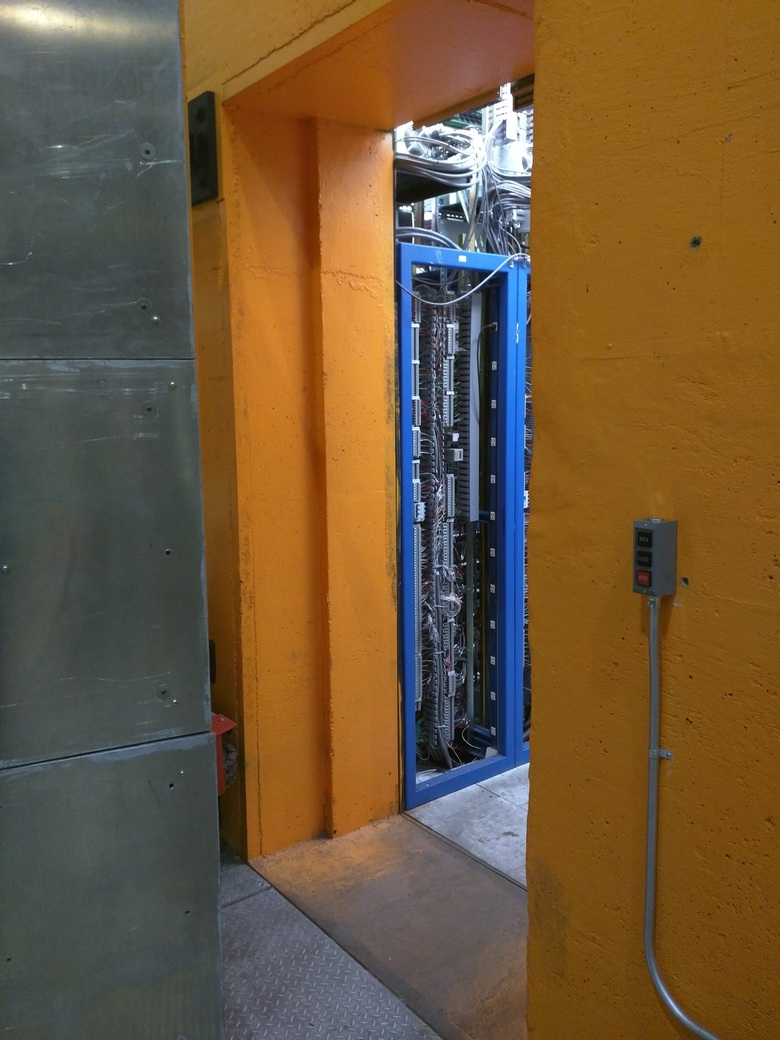
\includegraphics[width=4in]{shmsdoor.jpg}
\caption{\label{fig:shmsdoorcontrol}SHMS hut outside door control buttons.}
\end{center}
\end{figure}

\begin{figure}
\begin{center}
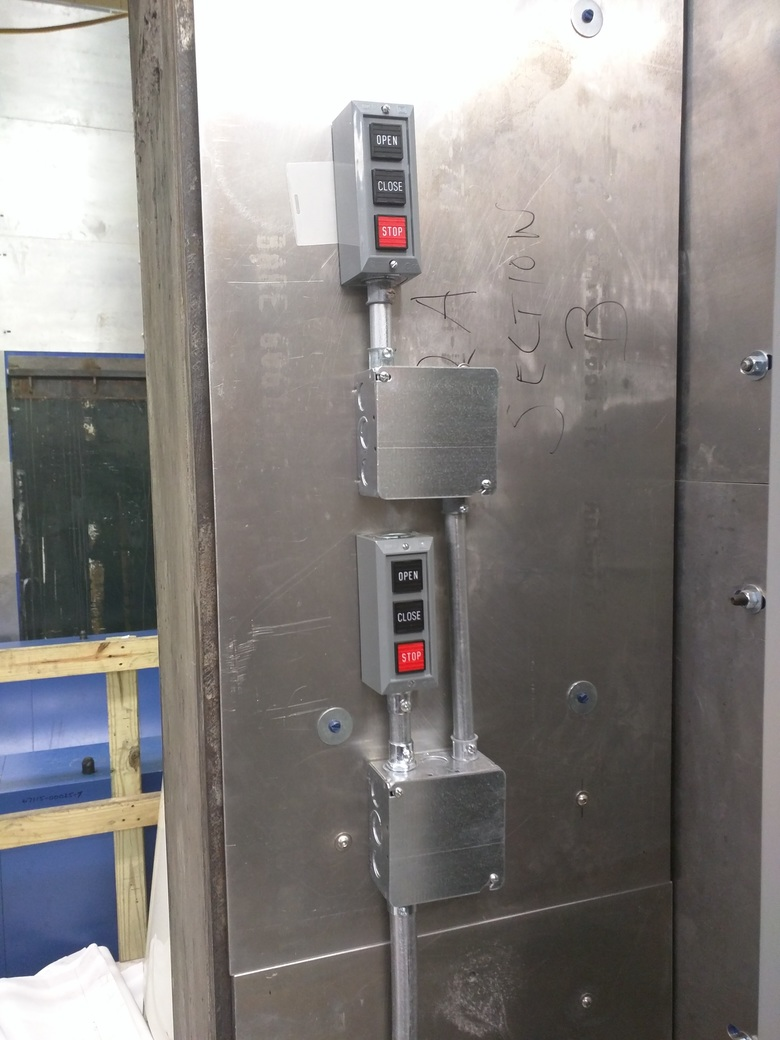
\includegraphics[width=3in]{barndoor-outside.jpg}
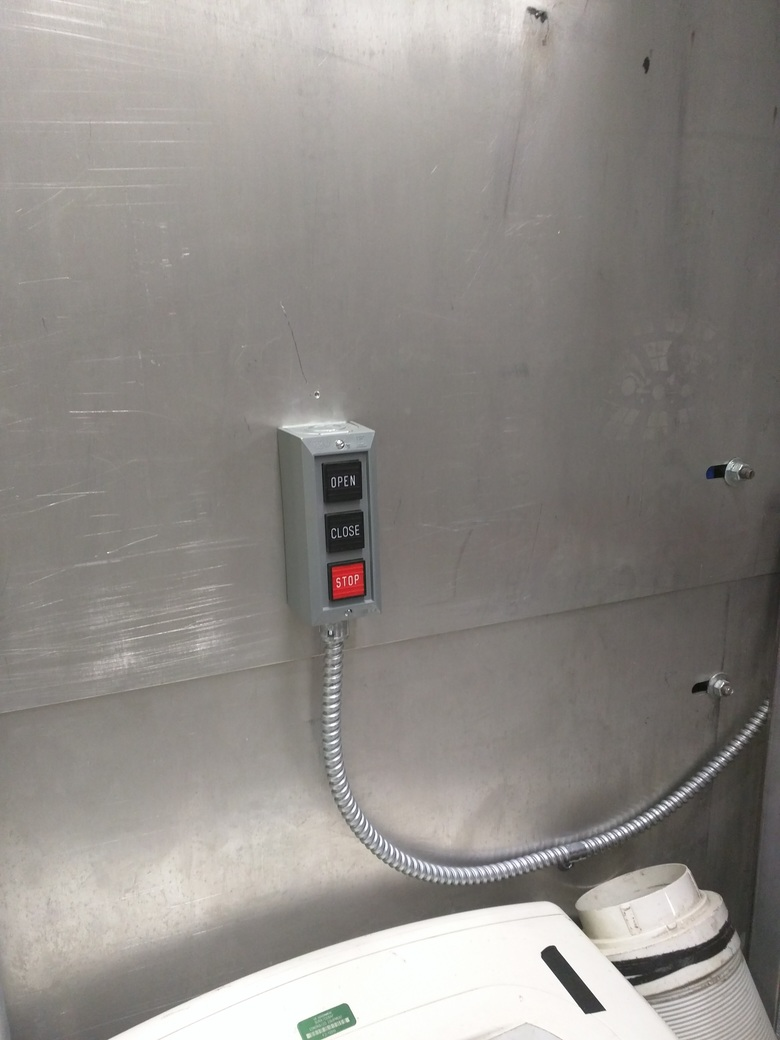
\includegraphics[width=3in]{barndoor-inside.jpg}
\caption{\label{fig:barndoorcontrol}SHMS barn door controls.  The left
  picture shows the controls located in electronics hut.  The bottom
  buttons control the barn door and the top buttons control the SHMS
  vacuum shutter.  The right picture shows the barn door controls
  located inside the detector hut.}
\end{center}
\end{figure}

\subsection{Drift Chambers}

\paragraph{Gas Flow Operating Procedures}
\sawnote{This may be common with enough the HMS that it can be moved
  into common chapter.  Or put common stuff (gas shed) in common
  section and hut details in spectrometer specific sections.}

\paragraph{Electronics Operating Procedures}
\sawnote{Description of drift chamber electronics and turn on procedure.
Threshold, +/-5V, VME crate(s).}

\subsection{Hodoscope}
The SHMS hodoscope consists of 4 planes, the first three made of bars
of scintillating plastic, and the fourth of synthetic quartz.
\sawnote{Should this be combined with HMS or be entirely separate.}
\sawnote{Check that Positive/Negative convention is the same.}

\subsubsection{Scintillator Hodoscope Planes}
Further information about the scintillator hodoscope planes, S1X, S2X,
and S1Y can be found in the ``SHMS Hodoscope Scintillator Detectors''
reference~\cite{howto:shms_scintillator_hodoscope}.

\subsubsection{Quartz Bar Hodoscope Plane}
\sawnote{Quartz detector is positive HV.  Big difference from HMS.
  Probably have it's own section separate from HMS.}

\subsection{Noble Gas Cerenkov Detector}
\sawnote{This detector is only sometimes installed}




